\documentclass{amsbook}
\usepackage{../amsTurkish}
\usepackage{../Ceyhun}
\usepackage{graphicx}
\usepackage{float}

\begin{document}
    \hPage{ceyhun/218}
    \begin{figure}[H]
    \footnote{used graphicx and float package}
      \centering
          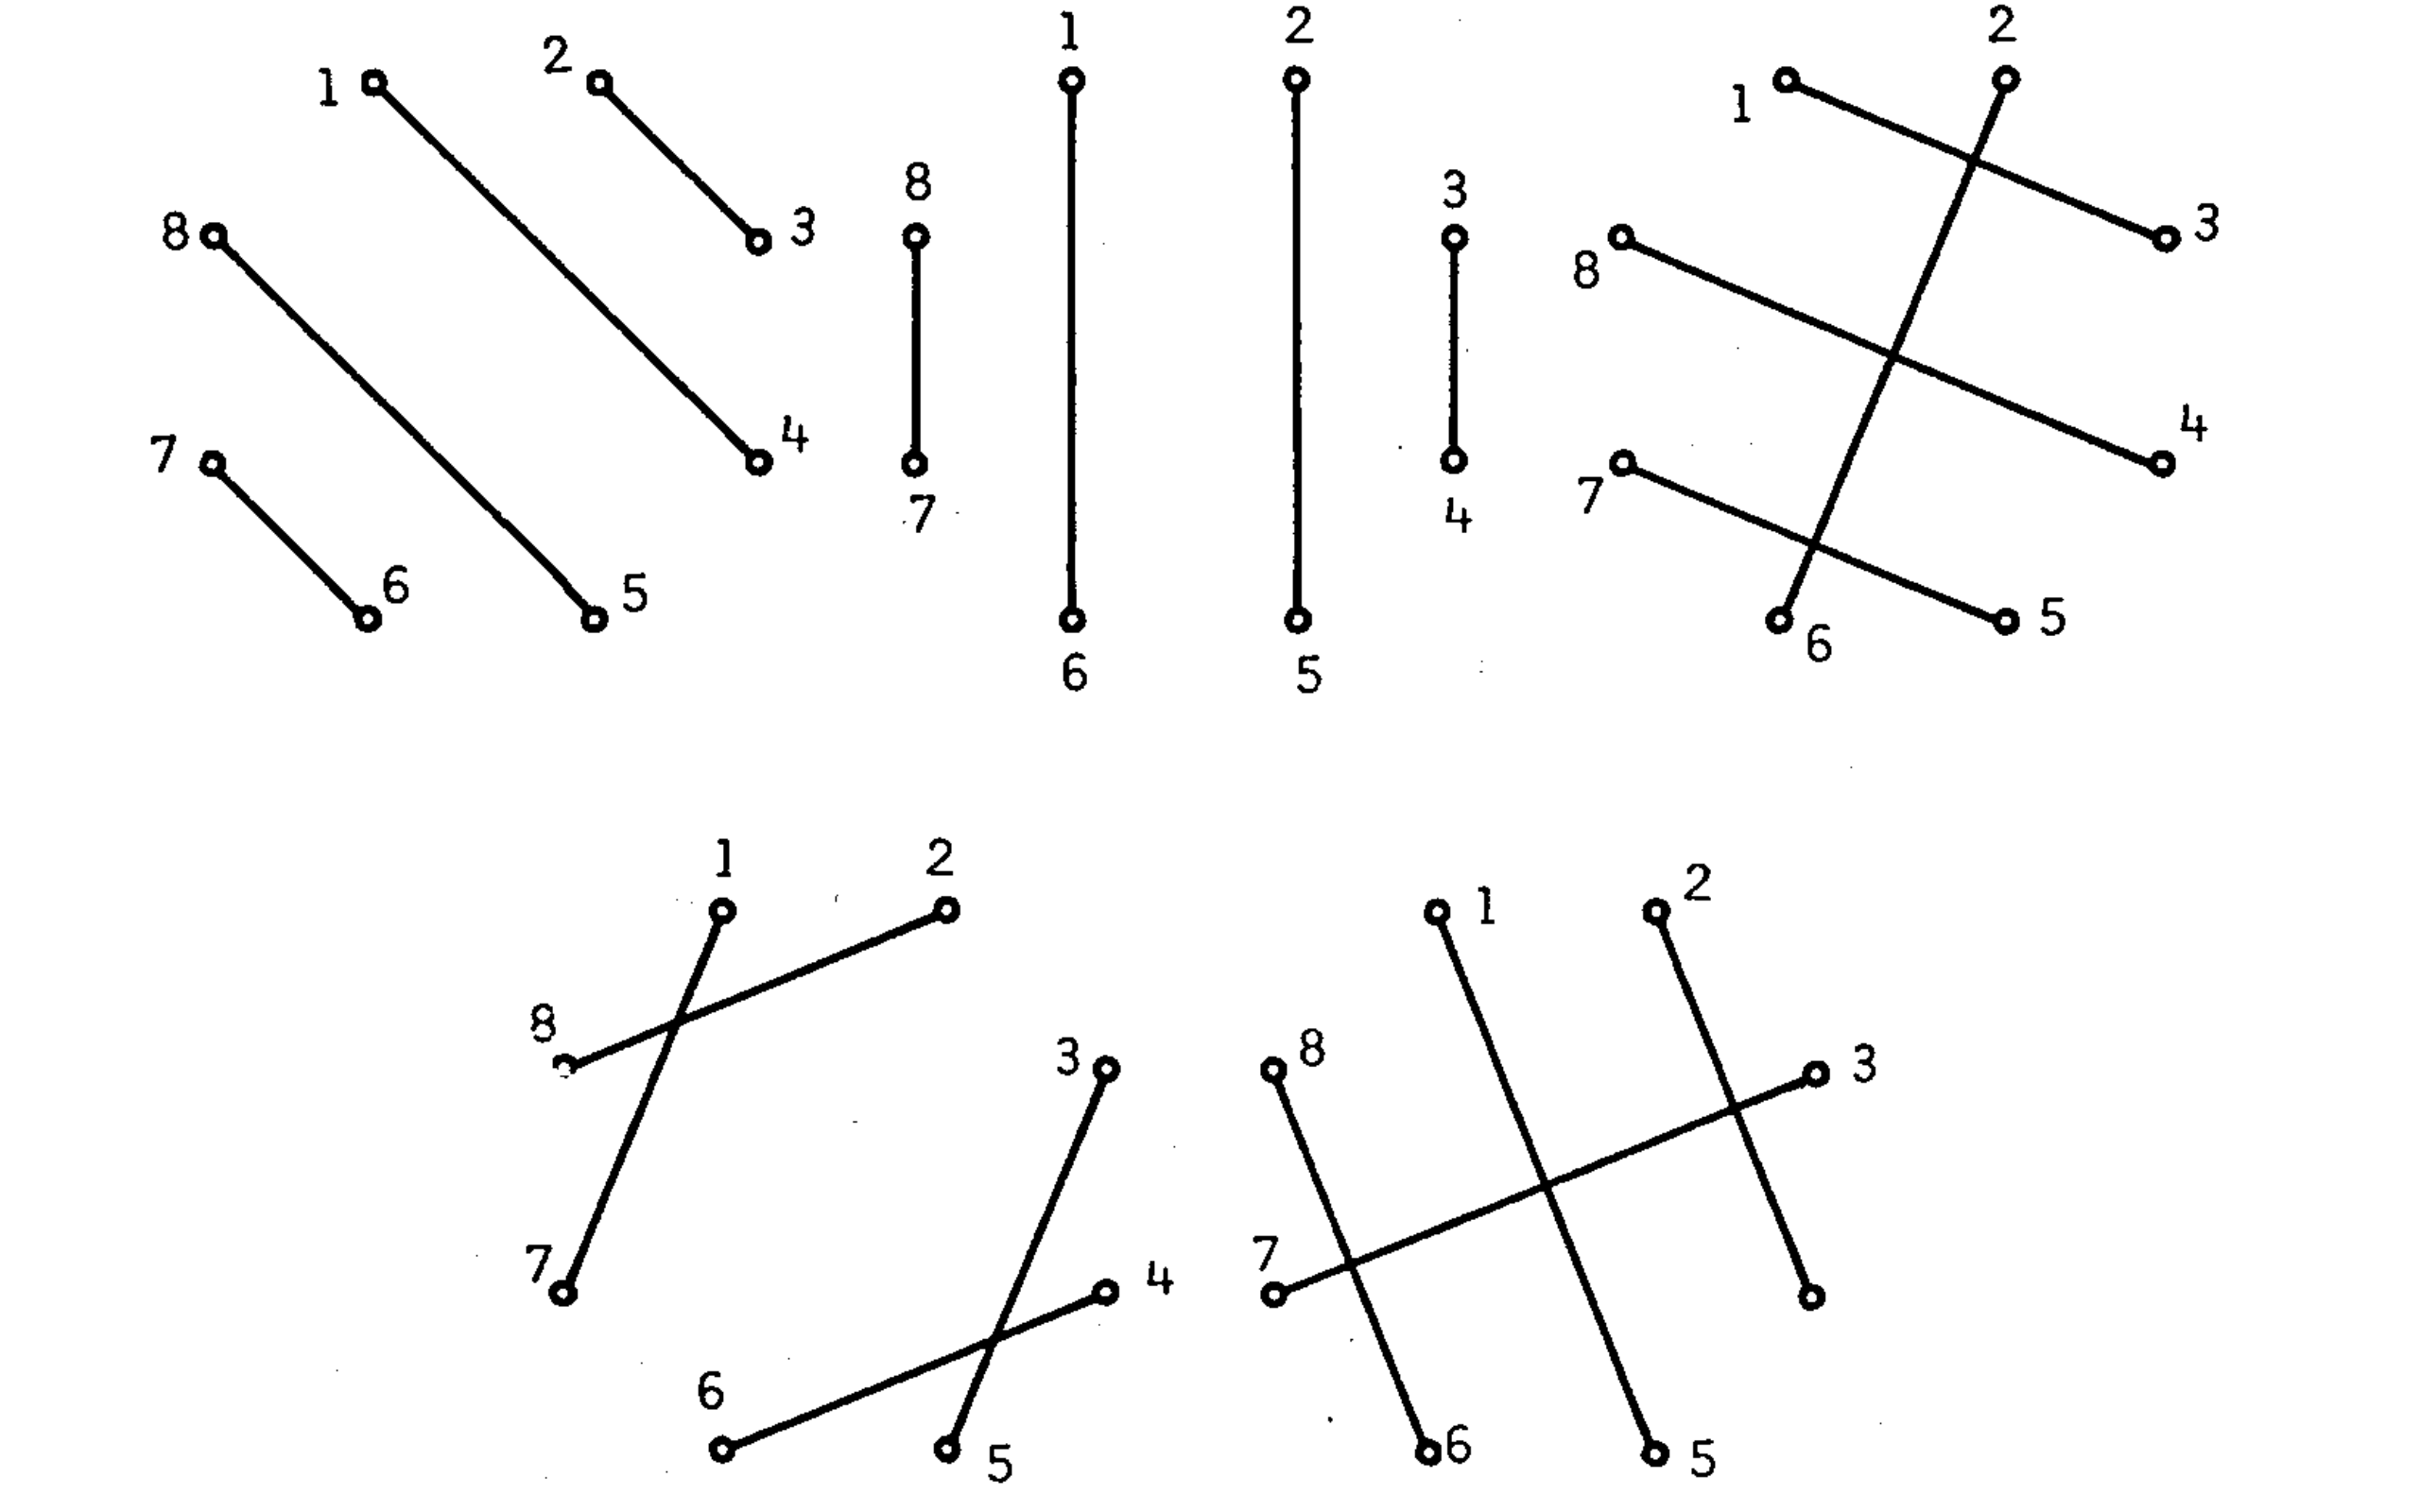
\includegraphics[width=1\textwidth]{images/ceyhun-218-fig01}
      \caption{1-ayrışır çizge ve 1-ayrışımı}
    \end{figure}
    Genel bir çizgede, 1-ayrığın varlığını\footnote{imla hatası düzeltildi} saptamak için aşağıdaki teoremi tanıtlamadan vereceğiz.
    \begin{theorem}
    Düğümlerinin toplamı çift sayı olan $Ç(d, a)$ çizgesinde en az bir 1-ayrığın bulunması için gerek ve yeter koşul; h sayıda düğümden oluşan bir düğüm kümesi çizgeden çıkarıldığında geriye kalan çizgede, düğümleri tek sayıya eşit parçaların sayısının $h$'den çok olmamasıdır.
    \end{theorem}
\end{document}
